% generated by Plantuml 1.2024.3       
\definecolor{plantucolor0000}{RGB}{0,0,0}
\definecolor{plantucolor0001}{RGB}{255,192,203}
\definecolor{plantucolor0002}{RGB}{173,216,230}
\definecolor{plantucolor0003}{RGB}{255,255,255}
\definecolor{plantucolor0004}{RGB}{24,24,24}
\definecolor{plantucolor0005}{RGB}{232,232,255}
\definecolor{plantucolor0006}{RGB}{255,234,213}
\definecolor{plantucolor0007}{RGB}{213,255,213}
\definecolor{plantucolor0008}{RGB}{255,232,232}
\definecolor{plantucolor0009}{RGB}{238,238,238}
\definecolor{plantucolor0010}{RGB}{254,255,221}
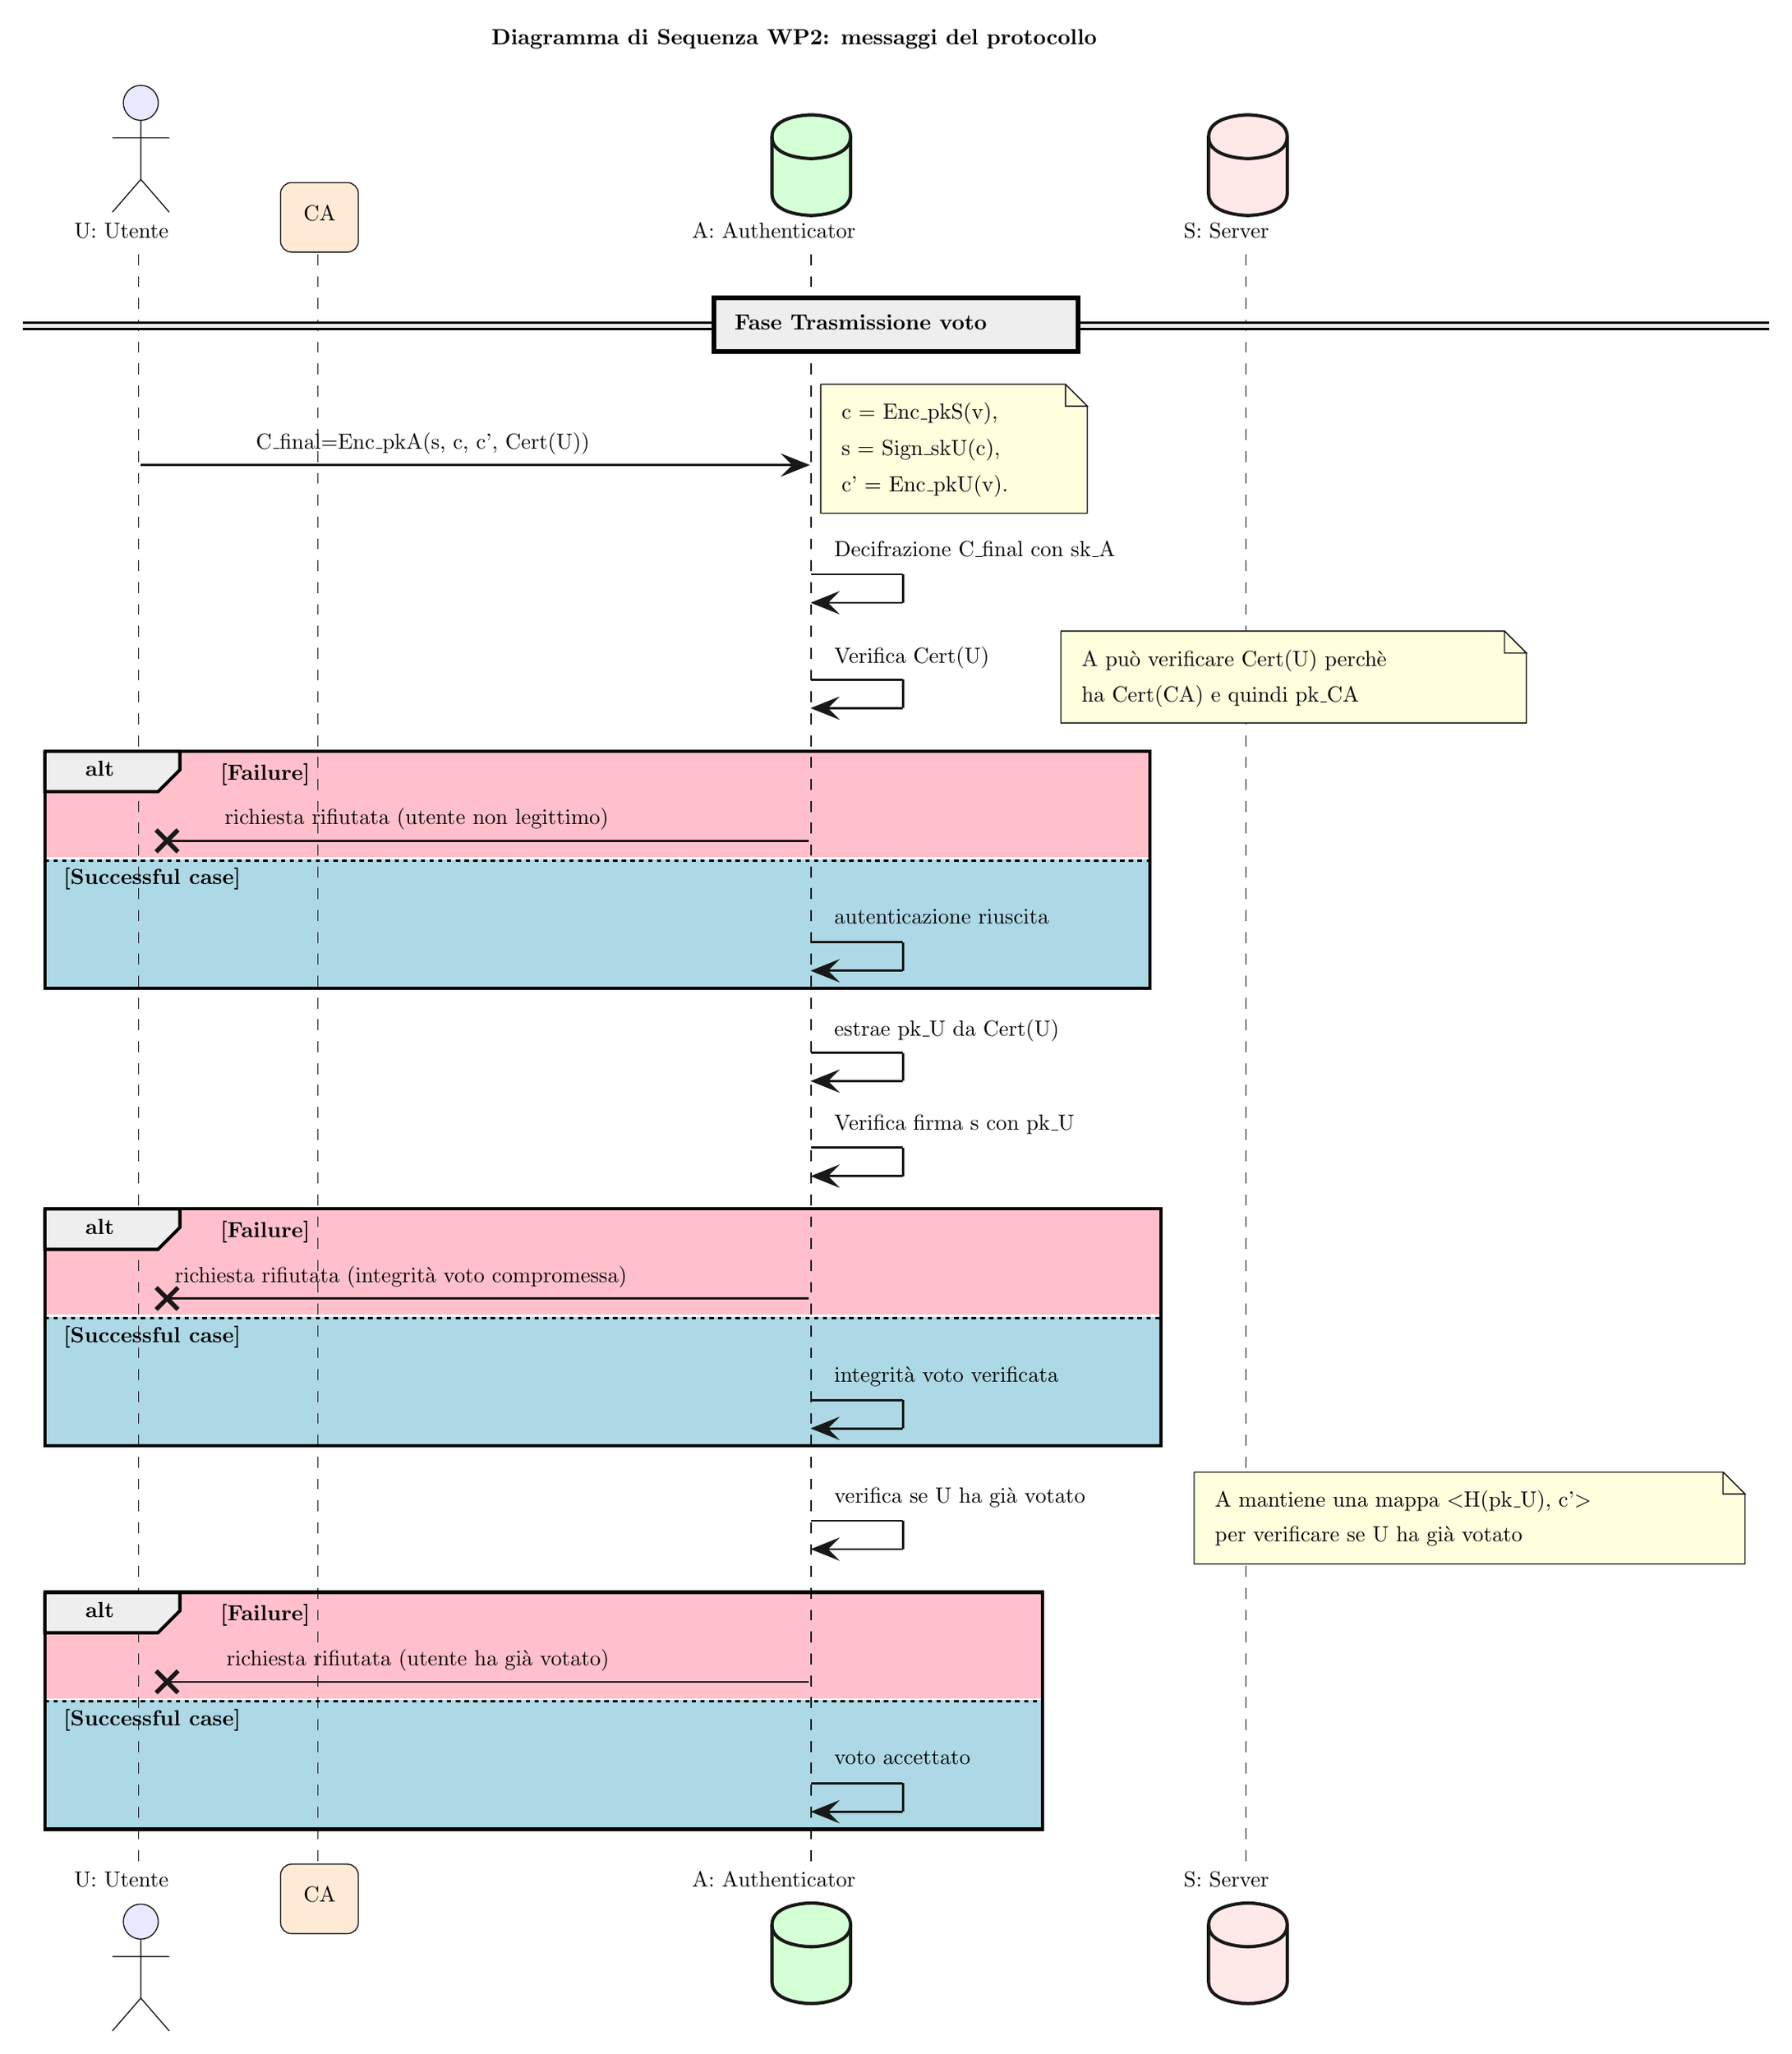
\begin{tikzpicture}[yscale=-1
,pstyle0/.style={color=black,fill=plantucolor0001,line width=1.5pt}
,pstyle1/.style={color=plantucolor0003,fill=plantucolor0002,line width=1.0pt}
,pstyle2/.style={color=plantucolor0004,line width=0.5pt,dash pattern=on 5.0pt off 5.0pt}
,pstyle3/.style={color=plantucolor0004,fill=plantucolor0005,line width=0.5pt}
,pstyle4/.style={color=plantucolor0004,line width=0.5pt}
,pstyle5/.style={color=plantucolor0004,fill=plantucolor0006,line width=0.5pt}
,pstyle6/.style={color=plantucolor0004,fill=plantucolor0007,line width=1.5pt}
,pstyle7/.style={color=plantucolor0004,line width=1.5pt}
,pstyle8/.style={color=plantucolor0004,fill=plantucolor0008,line width=1.5pt}
,pstyle10/.style={color=black,line width=1.0pt}
,pstyle12/.style={color=plantucolor0004,fill=plantucolor0004,line width=1.0pt}
,pstyle13/.style={color=plantucolor0004,line width=1.0pt}
,pstyle14/.style={color=plantucolor0004,fill=plantucolor0010,line width=0.5pt}
,pstyle15/.style={color=black,fill=plantucolor0009,line width=1.5pt}
,pstyle16/.style={color=black,line width=1.5pt}
,pstyle17/.style={color=plantucolor0004,line width=2.0pt}
,pstyle18/.style={color=black,line width=1.0pt,dash pattern=on 2.0pt off 2.0pt}
]
\node at (210.8648pt,15pt)[below right,color=black]{\textbf{Diagramma di Sequenza WP2: messaggi del protocollo}};
\draw[pstyle0] (10pt,348.8418pt) rectangle (515.6349pt,457.2207pt);
\draw[pstyle1] (10pt,397.7988pt) rectangle (515.6349pt,457.2207pt);
\draw[pstyle0] (10pt,558.1777pt) rectangle (520.5243pt,666.5566pt);
\draw[pstyle1] (10pt,607.1348pt) rectangle (520.5243pt,666.5566pt);
\draw[pstyle0] (10pt,733.5137pt) rectangle (466.4817pt,841.8926pt);
\draw[pstyle1] (10pt,782.4707pt) rectangle (466.4817pt,841.8926pt);
\draw[pstyle2] (53pt,121.4922pt) -- (53pt,858.8926pt);
\draw[pstyle2] (134.8615pt,121.4922pt) -- (134.8615pt,858.8926pt);
\draw[pstyle2] (360.6442pt,121.4922pt) -- (360.6442pt,858.8926pt);
\draw[pstyle2] (559.5962pt,121.4922pt) -- (559.5962pt,858.8926pt);
\node at (20pt,103.7461pt)[below right,color=black]{U: Utente};
\draw[pstyle3] (53.9308pt,52.2461pt) ellipse (8pt and 8pt);
\draw[pstyle4] (53.9308pt,60.2461pt) -- (53.9308pt,87.2461pt)(40.9308pt,68.2461pt) -- (66.9308pt,68.2461pt)(53.9308pt,87.2461pt) -- (40.9308pt,102.2461pt)(53.9308pt,87.2461pt) -- (66.9308pt,102.2461pt);
\node at (20pt,857.8926pt)[below right,color=black]{U: Utente};
\draw[pstyle3] (53.9308pt,884.1387pt) ellipse (8pt and 8pt);
\draw[pstyle4] (53.9308pt,892.1387pt) -- (53.9308pt,919.1387pt)(40.9308pt,900.1387pt) -- (66.9308pt,900.1387pt)(53.9308pt,919.1387pt) -- (40.9308pt,934.1387pt)(53.9308pt,919.1387pt) -- (66.9308pt,934.1387pt);
\draw[pstyle5] (117.8615pt,93.7461pt) arc (180:270:5pt) -- (122.8615pt,88.7461pt) -- (148.4615pt,88.7461pt) arc (270:360:5pt) -- (153.4615pt,93.7461pt) -- (153.4615pt,115.4922pt) arc (0:90:5pt) -- (148.4615pt,120.4922pt) -- (122.8615pt,120.4922pt) arc (90:180:5pt) -- (117.8615pt,115.4922pt) -- cycle;
\node at (124.8615pt,95.7461pt)[below right,color=black]{CA};
\draw[pstyle5] (117.8615pt,862.8926pt) arc (180:270:5pt) -- (122.8615pt,857.8926pt) -- (148.4615pt,857.8926pt) arc (270:360:5pt) -- (153.4615pt,862.8926pt) -- (153.4615pt,884.6387pt) arc (0:90:5pt) -- (148.4615pt,889.6387pt) -- (122.8615pt,889.6387pt) arc (90:180:5pt) -- (117.8615pt,884.6387pt) -- cycle;
\node at (124.8615pt,864.8926pt)[below right,color=black]{CA};
\node at (302.6442pt,103.7461pt)[below right,color=black]{A: Authenticator};
\draw[pstyle6] (342.6921pt,67.7461pt) ..controls (342.6921pt,57.7461pt) and (360.6921pt,57.7461pt) .. (360.6921pt,57.7461pt) ..controls (360.6921pt,57.7461pt) and (378.6921pt,57.7461pt) .. (378.6921pt,67.7461pt) -- (378.6921pt,93.7461pt) ..controls (378.6921pt,103.7461pt) and (360.6921pt,103.7461pt) .. (360.6921pt,103.7461pt) ..controls (360.6921pt,103.7461pt) and (342.6921pt,103.7461pt) .. (342.6921pt,93.7461pt) -- (342.6921pt,67.7461pt);
\draw[pstyle7] (342.6921pt,67.7461pt) ..controls (342.6921pt,77.7461pt) and (360.6921pt,77.7461pt) .. (360.6921pt,77.7461pt) ..controls (360.6921pt,77.7461pt) and (378.6921pt,77.7461pt) .. (378.6921pt,67.7461pt);
\node at (302.6442pt,857.8926pt)[below right,color=black]{A: Authenticator};
\draw[pstyle6] (342.6921pt,885.6387pt) ..controls (342.6921pt,875.6387pt) and (360.6921pt,875.6387pt) .. (360.6921pt,875.6387pt) ..controls (360.6921pt,875.6387pt) and (378.6921pt,875.6387pt) .. (378.6921pt,885.6387pt) -- (378.6921pt,911.6387pt) ..controls (378.6921pt,921.6387pt) and (360.6921pt,921.6387pt) .. (360.6921pt,921.6387pt) ..controls (360.6921pt,921.6387pt) and (342.6921pt,921.6387pt) .. (342.6921pt,911.6387pt) -- (342.6921pt,885.6387pt);
\draw[pstyle7] (342.6921pt,885.6387pt) ..controls (342.6921pt,895.6387pt) and (360.6921pt,895.6387pt) .. (360.6921pt,895.6387pt) ..controls (360.6921pt,895.6387pt) and (378.6921pt,895.6387pt) .. (378.6921pt,885.6387pt);
\node at (527.5962pt,103.7461pt)[below right,color=black]{S: Server};
\draw[pstyle8] (542.4501pt,67.7461pt) ..controls (542.4501pt,57.7461pt) and (560.4501pt,57.7461pt) .. (560.4501pt,57.7461pt) ..controls (560.4501pt,57.7461pt) and (578.4501pt,57.7461pt) .. (578.4501pt,67.7461pt) -- (578.4501pt,93.7461pt) ..controls (578.4501pt,103.7461pt) and (560.4501pt,103.7461pt) .. (560.4501pt,103.7461pt) ..controls (560.4501pt,103.7461pt) and (542.4501pt,103.7461pt) .. (542.4501pt,93.7461pt) -- (542.4501pt,67.7461pt);
\draw[pstyle7] (542.4501pt,67.7461pt) ..controls (542.4501pt,77.7461pt) and (560.4501pt,77.7461pt) .. (560.4501pt,77.7461pt) ..controls (560.4501pt,77.7461pt) and (578.4501pt,77.7461pt) .. (578.4501pt,67.7461pt);
\node at (527.5962pt,857.8926pt)[below right,color=black]{S: Server};
\draw[pstyle8] (542.4501pt,885.6387pt) ..controls (542.4501pt,875.6387pt) and (560.4501pt,875.6387pt) .. (560.4501pt,875.6387pt) ..controls (560.4501pt,875.6387pt) and (578.4501pt,875.6387pt) .. (578.4501pt,885.6387pt) -- (578.4501pt,911.6387pt) ..controls (578.4501pt,921.6387pt) and (560.4501pt,921.6387pt) .. (560.4501pt,921.6387pt) ..controls (560.4501pt,921.6387pt) and (542.4501pt,921.6387pt) .. (542.4501pt,911.6387pt) -- (542.4501pt,885.6387pt);
\draw[pstyle7] (542.4501pt,885.6387pt) ..controls (542.4501pt,895.6387pt) and (560.4501pt,895.6387pt) .. (560.4501pt,895.6387pt) ..controls (560.4501pt,895.6387pt) and (578.4501pt,895.6387pt) .. (578.4501pt,885.6387pt);
\draw[color=plantucolor0009,fill=plantucolor0009,line width=1.0pt] (0pt,152.7314pt) rectangle (798.7861pt,155.7314pt);
\draw[pstyle10] (0pt,152.7314pt) -- (798.7861pt,152.7314pt);
\draw[pstyle10] (0pt,155.7314pt) -- (798.7861pt,155.7314pt);
\draw[color=black,fill=plantucolor0009,line width=2.0pt] (316.0854pt,141.4922pt) rectangle (482.7007pt,165.9707pt);
\node at (322.0854pt,145.4922pt)[below right,color=black]{\textbf{Fase Trasmissione voto }};
\draw[pstyle12] (348.6921pt,213.9277pt) -- (358.6921pt,217.9277pt) -- (348.6921pt,221.9277pt) -- (352.6921pt,217.9277pt) -- cycle;
\draw[pstyle13] (53.9308pt,217.9277pt) -- (354.6921pt,217.9277pt);
\node at (103.1003pt,199.4492pt)[below right,color=black]{C\_final=Enc\_pkA(s, c, c', Cert(U))};
\draw[pstyle14] (365pt,180.9707pt) -- (365pt,239.9707pt) -- (487pt,239.9707pt) -- (487pt,190.9707pt) -- (477pt,180.9707pt) -- (365pt,180.9707pt);
\draw[pstyle14] (477pt,180.9707pt) -- (477pt,190.9707pt) -- (487pt,190.9707pt) -- (477pt,180.9707pt);
\node at (371pt,185.9707pt)[below right,color=black]{c = Enc\_pkS(v),};
\node at (371pt,202.4492pt)[below right,color=black]{s = Sign\_skU(c),};
\node at (371pt,218.9277pt)[below right,color=black]{c' = Enc\_pkU(v).};
\draw[pstyle13] (360.6921pt,267.8848pt) -- (402.6921pt,267.8848pt);
\draw[pstyle13] (402.6921pt,267.8848pt) -- (402.6921pt,280.8848pt);
\draw[pstyle13] (361.6921pt,280.8848pt) -- (402.6921pt,280.8848pt);
\draw[pstyle12] (371.6921pt,276.8848pt) -- (361.6921pt,280.8848pt) -- (371.6921pt,284.8848pt) -- (367.6921pt,280.8848pt) -- cycle;
\node at (367.6921pt,249.4063pt)[below right,color=black]{Decifrazione C\_final con sk\_A};
\draw[pstyle13] (360.6921pt,316.1025pt) -- (402.6921pt,316.1025pt);
\draw[pstyle13] (402.6921pt,316.1025pt) -- (402.6921pt,329.1025pt);
\draw[pstyle13] (361.6921pt,329.1025pt) -- (402.6921pt,329.1025pt);
\draw[pstyle12] (371.6921pt,325.1025pt) -- (361.6921pt,329.1025pt) -- (371.6921pt,333.1025pt) -- (367.6921pt,329.1025pt) -- cycle;
\node at (367.6921pt,297.624pt)[below right,color=black]{Verifica Cert(U)};
\draw[pstyle14] (474.8634pt,293.8848pt) -- (474.8634pt,335.8848pt) -- (687.8634pt,335.8848pt) -- (687.8634pt,303.8848pt) -- (677.8634pt,293.8848pt) -- (474.8634pt,293.8848pt);
\draw[pstyle14] (677.8634pt,293.8848pt) -- (677.8634pt,303.8848pt) -- (687.8634pt,303.8848pt) -- (677.8634pt,293.8848pt);
\node at (480.8634pt,298.8848pt)[below right,color=black]{A può verificare Cert(U) perchè};
\node at (480.8634pt,315.3633pt)[below right,color=black]{ha Cert(CA) e quindi pk\_CA};
\draw[pstyle15] (10pt,348.8418pt) -- (71.8pt,348.8418pt) -- (71.8pt,357.3203pt) -- (61.8pt,367.3203pt) -- (10pt,367.3203pt) -- (10pt,348.8418pt);
\draw[pstyle16] (10pt,348.8418pt) rectangle (515.6349pt,457.2207pt);
\node at (25pt,349.8418pt)[below right,color=black]{\textbf{alt}};
\node at (86.8pt,350.8418pt)[below right,color=black]{\textbf{[Failure]}};
\draw[pstyle17] (60.9308pt,384.7988pt) -- (70.9308pt,394.7988pt);
\draw[pstyle17] (60.9308pt,394.7988pt) -- (70.9308pt,384.7988pt);
\draw[pstyle13] (65.9308pt,389.7988pt) -- (359.6921pt,389.7988pt);
\node at (88.8022pt,371.3203pt)[below right,color=black]{richiesta rifiutata (utente non legittimo)};
\draw[pstyle18] (10pt,398.7988pt) -- (515.6349pt,398.7988pt);
\node at (15pt,398.7988pt)[below right,color=black]{\textbf{[Successful case]}};
\draw[pstyle13] (360.6921pt,436.2207pt) -- (402.6921pt,436.2207pt);
\draw[pstyle13] (402.6921pt,436.2207pt) -- (402.6921pt,449.2207pt);
\draw[pstyle13] (361.6921pt,449.2207pt) -- (402.6921pt,449.2207pt);
\draw[pstyle12] (371.6921pt,445.2207pt) -- (361.6921pt,449.2207pt) -- (371.6921pt,453.2207pt) -- (367.6921pt,449.2207pt) -- cycle;
\node at (367.6921pt,417.7422pt)[below right,color=black]{autenticazione riuscita};
\draw[pstyle13] (360.6921pt,486.6992pt) -- (402.6921pt,486.6992pt);
\draw[pstyle13] (402.6921pt,486.6992pt) -- (402.6921pt,499.6992pt);
\draw[pstyle13] (361.6921pt,499.6992pt) -- (402.6921pt,499.6992pt);
\draw[pstyle12] (371.6921pt,495.6992pt) -- (361.6921pt,499.6992pt) -- (371.6921pt,503.6992pt) -- (367.6921pt,499.6992pt) -- cycle;
\node at (367.6921pt,468.2207pt)[below right,color=black]{estrae pk\_U da Cert(U)};
\draw[pstyle13] (360.6921pt,530.1777pt) -- (402.6921pt,530.1777pt);
\draw[pstyle13] (402.6921pt,530.1777pt) -- (402.6921pt,543.1777pt);
\draw[pstyle13] (361.6921pt,543.1777pt) -- (402.6921pt,543.1777pt);
\draw[pstyle12] (371.6921pt,539.1777pt) -- (361.6921pt,543.1777pt) -- (371.6921pt,547.1777pt) -- (367.6921pt,543.1777pt) -- cycle;
\node at (367.6921pt,511.6992pt)[below right,color=black]{Verifica firma s con pk\_U};
\draw[pstyle15] (10pt,558.1777pt) -- (71.8pt,558.1777pt) -- (71.8pt,566.6563pt) -- (61.8pt,576.6563pt) -- (10pt,576.6563pt) -- (10pt,558.1777pt);
\draw[pstyle16] (10pt,558.1777pt) rectangle (520.5243pt,666.5566pt);
\node at (25pt,559.1777pt)[below right,color=black]{\textbf{alt}};
\node at (86.8pt,560.1777pt)[below right,color=black]{\textbf{[Failure]}};
\draw[pstyle17] (60.9308pt,594.1348pt) -- (70.9308pt,604.1348pt);
\draw[pstyle17] (60.9308pt,604.1348pt) -- (70.9308pt,594.1348pt);
\draw[pstyle13] (65.9308pt,599.1348pt) -- (359.6921pt,599.1348pt);
\node at (65.9308pt,580.6563pt)[below right,color=black]{richiesta rifiutata (integrità voto compromessa)};
\draw[pstyle18] (10pt,608.1348pt) -- (520.5243pt,608.1348pt);
\node at (15pt,608.1348pt)[below right,color=black]{\textbf{[Successful case]}};
\draw[pstyle13] (360.6921pt,645.5566pt) -- (402.6921pt,645.5566pt);
\draw[pstyle13] (402.6921pt,645.5566pt) -- (402.6921pt,658.5566pt);
\draw[pstyle13] (361.6921pt,658.5566pt) -- (402.6921pt,658.5566pt);
\draw[pstyle12] (371.6921pt,654.5566pt) -- (361.6921pt,658.5566pt) -- (371.6921pt,662.5566pt) -- (367.6921pt,658.5566pt) -- cycle;
\node at (367.6921pt,627.0781pt)[below right,color=black]{integrità voto verificata};
\draw[pstyle13] (360.6921pt,700.7744pt) -- (402.6921pt,700.7744pt);
\draw[pstyle13] (402.6921pt,700.7744pt) -- (402.6921pt,713.7744pt);
\draw[pstyle13] (361.6921pt,713.7744pt) -- (402.6921pt,713.7744pt);
\draw[pstyle12] (371.6921pt,709.7744pt) -- (361.6921pt,713.7744pt) -- (371.6921pt,717.7744pt) -- (367.6921pt,713.7744pt) -- cycle;
\node at (367.6921pt,682.2959pt)[below right,color=black]{verifica se U ha già votato};
\draw[pstyle14] (535.8719pt,678.5566pt) -- (535.8719pt,720.5566pt) -- (787.8719pt,720.5566pt) -- (787.8719pt,688.5566pt) -- (777.8719pt,678.5566pt) -- (535.8719pt,678.5566pt);
\draw[pstyle14] (777.8719pt,678.5566pt) -- (777.8719pt,688.5566pt) -- (787.8719pt,688.5566pt) -- (777.8719pt,678.5566pt);
\node at (541.8719pt,683.5566pt)[below right,color=black]{A mantiene una mappa \textless H(pk\_U), c'\textgreater };
\node at (541.8719pt,700.0352pt)[below right,color=black]{per verificare se U ha già votato};
\draw[pstyle15] (10pt,733.5137pt) -- (71.8pt,733.5137pt) -- (71.8pt,741.9922pt) -- (61.8pt,751.9922pt) -- (10pt,751.9922pt) -- (10pt,733.5137pt);
\draw[pstyle16] (10pt,733.5137pt) rectangle (466.4817pt,841.8926pt);
\node at (25pt,734.5137pt)[below right,color=black]{\textbf{alt}};
\node at (86.8pt,735.5137pt)[below right,color=black]{\textbf{[Failure]}};
\draw[pstyle17] (60.9308pt,769.4707pt) -- (70.9308pt,779.4707pt);
\draw[pstyle17] (60.9308pt,779.4707pt) -- (70.9308pt,769.4707pt);
\draw[pstyle13] (65.9308pt,774.4707pt) -- (359.6921pt,774.4707pt);
\node at (89.6042pt,755.9922pt)[below right,color=black]{richiesta rifiutata (utente ha già votato)};
\draw[pstyle18] (10pt,783.4707pt) -- (466.4817pt,783.4707pt);
\node at (15pt,783.4707pt)[below right,color=black]{\textbf{[Successful case]}};
\draw[pstyle13] (360.6921pt,820.8926pt) -- (402.6921pt,820.8926pt);
\draw[pstyle13] (402.6921pt,820.8926pt) -- (402.6921pt,833.8926pt);
\draw[pstyle13] (361.6921pt,833.8926pt) -- (402.6921pt,833.8926pt);
\draw[pstyle12] (371.6921pt,829.8926pt) -- (361.6921pt,833.8926pt) -- (371.6921pt,837.8926pt) -- (367.6921pt,833.8926pt) -- cycle;
\node at (367.6921pt,802.4141pt)[below right,color=black]{voto accettato};
\end{tikzpicture}
